\chapter{Free-Space Path Loss (FSPL)}
\label{ch:fspl}

\begin{nontechnical}
\textbf{Like shouting across a field---the farther away, the quieter. Radio waves spread out and weaken with distance.}

\textbf{Simple idea:}
\begin{itemize}
\item \textbf{Double the distance} = signal becomes \textbf{4$\times$ weaker}
\item \textbf{Higher frequency} (5G) = weaker than lower frequency (4G) over same distance
\item \textbf{Satellites 36,000~km away}: Signal weakens by 10 trillion trillion times! (That's why dishes are big)
\end{itemize}

\textbf{Real examples:} WiFi weakens 10,000$\times$ over 50~meters. Cell towers need to be closer for 5G than 4G.

\textbf{Why does this matter?} It tells engineers how much power to use and how big to make antennas. It's the starting point for designing any wireless link.
\end{nontechnical}

\section{Overview}

\textbf{Free-Space Path Loss (FSPL)} quantifies the reduction in signal power as an electromagnetic wave propagates through free space.

\begin{keyconcept}
FSPL is \textbf{not energy dissipation}---it's geometric spreading. The total radiated power remains constant, but power density decreases as the wave expands over a spherical surface of area $4\pi d^2$. This fundamental relationship drives all wireless link budget calculations.
\end{keyconcept}

FSPL provides the baseline loss for any wireless communication link. In practice, additional losses from atmosphere, multipath, obstacles, and hardware imperfections add to this fundamental limit.

\section{The Friis Transmission Equation}

The fundamental relationship linking transmit and receive power in free space:

\begin{equation}
P_R = P_T \cdot G_T \cdot G_R \cdot \left(\frac{\lambda}{4\pi d}\right)^2
\end{equation}
where:
\begin{itemize}
\item $P_R$ = received power (W)
\item $P_T$ = transmitted power (W)
\item $G_T$ = transmit antenna gain (linear, dimensionless)
\item $G_R$ = receive antenna gain (linear, dimensionless)
\item $\lambda$ = wavelength (m) = $c/f$ where $c = 3 \times 10^8$~m/s
\item $d$ = distance between antennas (m)
\end{itemize}

\textbf{Assumptions:}
\begin{itemize}
\item Free space (no obstacles, no atmosphere)
\item Far-field region: $d \gg$ antenna dimensions and $d \gg \lambda$
\item Polarization matched between transmitter and receiver
\item Antennas properly aligned
\end{itemize}

\subsection{Physical Interpretation}

The term $(\lambda/4\pi d)^2$ captures two fundamental concepts:

\textbf{1. Geometric spreading:} Power radiates spherically from an isotropic antenna. At distance $d$, the power is distributed over surface area $A_{\text{sphere}} = 4\pi d^2$, causing power density to drop as $1/d^2$.

\textbf{2. Effective aperture:} The receiving antenna captures power proportional to its effective area $A_{\text{eff}} = G_R \lambda^2 / 4\pi$. Higher frequencies (smaller $\lambda$) have smaller effective apertures, leading to greater loss.

\begin{center}
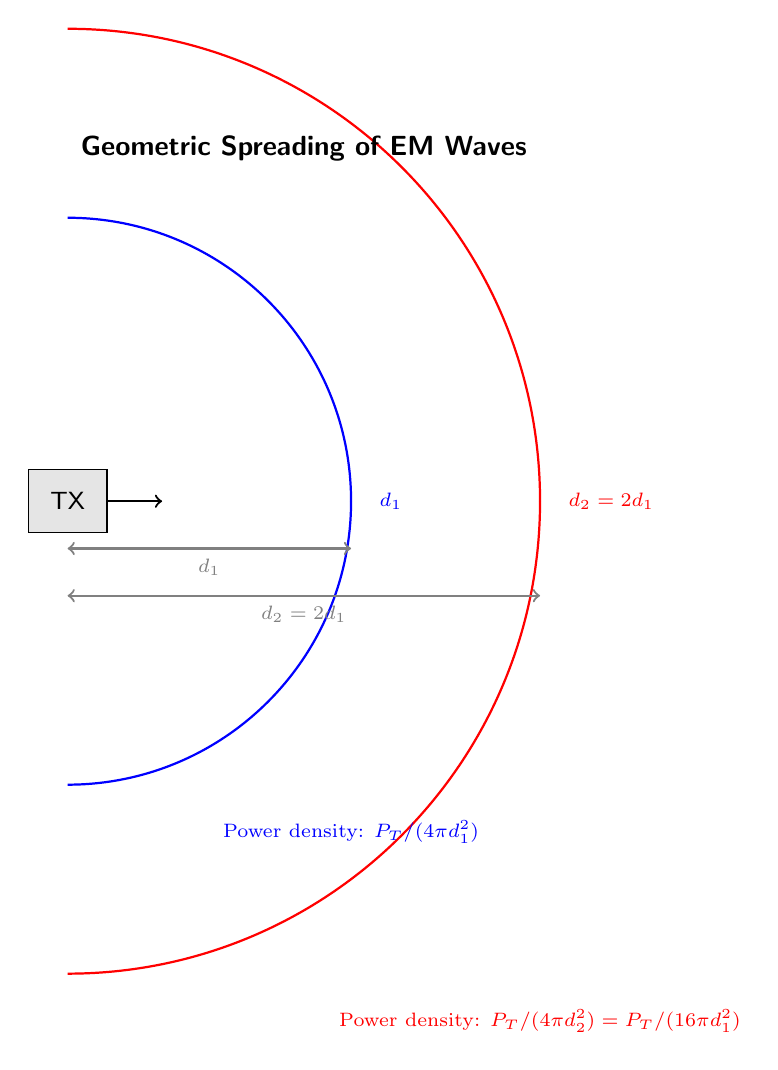
\begin{tikzpicture}[scale=1.2]
% Transmitter
\node[draw, rectangle, minimum width=1cm, minimum height=0.8cm, fill=black!10] (tx) at (0,0) {\sffamily\small TX};
\draw[->,thick] (tx) -- (1,0);

% Spherical wavefront at distance d1
\draw[thick, blue] (3,0) arc[start angle=0, end angle=90, radius=3cm];
\draw[thick, blue] (3,0) arc[start angle=0, end angle=-90, radius=3cm];
\node[blue, right] at (3.2,0) {\scriptsize $d_1$};

% Spherical wavefront at distance d2
\draw[thick, red] (5,0) arc[start angle=0, end angle=90, radius=5cm];
\draw[thick, red] (5,0) arc[start angle=0, end angle=-90, radius=5cm];
\node[red, right] at (5.2,0) {\scriptsize $d_2 = 2d_1$};

% Power density annotations
\node[blue] at (3,-3.5) {\scriptsize Power density: $P_T/(4\pi d_1^2)$};
\node[red] at (5,-5.5) {\scriptsize Power density: $P_T/(4\pi d_2^2) = P_T/(16\pi d_1^2)$};

% Title
\node[above] at (2.5,3.5) {\sffamily\bfseries Geometric Spreading of EM Waves};

% Distance markers
\draw[<->, thick, gray] (0,-0.5) -- (3,-0.5) node[midway, below] {\scriptsize $d_1$};
\draw[<->, thick, gray] (0,-1) -- (5,-1) node[midway, below] {\scriptsize $d_2 = 2d_1$};
\end{tikzpicture}
\end{center}

\begin{calloutbox}{Doubling Distance}
When distance doubles from $d_1$ to $2d_1$:
\begin{itemize}
\item Spherical surface area increases $4\times$: $(4\pi d_1^2) \rightarrow (4\pi [2d_1]^2) = 16\pi d_1^2$
\item Power density decreases to $1/4$ of original
\item In dB: $10\log_{10}(1/4) = -6$~dB loss
\end{itemize}
\end{calloutbox}

\section{FSPL Formulation}

\subsection{Path Loss Definition}

\textbf{Path Loss (L)} is defined as the ratio of transmitted to received power:

\begin{equation}
L = \frac{P_T}{P_R}
\end{equation}

In decibels:
\begin{equation}
L_{\text{dB}} = 10\log_{10}(L) = 10\log_{10}\left(\frac{P_T}{P_R}\right) = P_T[\text{dBm}] - P_R[\text{dBm}]
\end{equation}

\subsection{Derivation from Friis Equation}

Assuming isotropic antennas ($G_T = G_R = 1$), the Friis equation becomes:

\begin{equation}
P_R = P_T \left(\frac{\lambda}{4\pi d}\right)^2
\end{equation}

Therefore, the free-space path loss is:

\begin{equation}
L = \frac{P_T}{P_R} = \left(\frac{4\pi d}{\lambda}\right)^2
\end{equation}

Substituting $\lambda = c/f$ where $c = 3 \times 10^8$~m/s:

\begin{equation}
L = \left(\frac{4\pi f d}{c}\right)^2
\end{equation}

\subsection{FSPL in Decibels}

Converting to logarithmic form:

\begin{equation}
\text{FSPL}_{\text{dB}} = 10\log_{10}(L) = 20\log_{10}\left(\frac{4\pi d}{\lambda}\right)
\end{equation}

Expanding:
\begin{equation}
\text{FSPL}_{\text{dB}} = 20\log_{10}(d) + 20\log_{10}(f) + 20\log_{10}\left(\frac{4\pi}{c}\right)
\end{equation}

\textbf{Practical form} (frequency in Hz, distance in meters):

\begin{equation}
\text{FSPL}_{\text{dB}} = 20\log_{10}(d_{\text{m}}) + 20\log_{10}(f_{\text{Hz}}) + 92.45
\end{equation}

\textbf{Alternative form} (frequency in MHz, distance in km):

\begin{equation}
\text{FSPL}_{\text{dB}} = 20\log_{10}(d_{\text{km}}) + 20\log_{10}(f_{\text{MHz}}) + 32.45
\end{equation}

\begin{warningbox}
The constant term (92.45 or 32.45) depends on the units used. Always verify your units match the formula. Mixing units (e.g., using GHz with the MHz formula) introduces a $\pm 60$~dB error---enough to make a working link appear impossible or vice versa.
\end{warningbox}

\section{Scaling Laws}

\subsection{Distance Dependence}

From equation (9), FSPL increases with distance:

\begin{equation}
\text{FSPL} \propto d^2 \quad \text{(power law)}
\end{equation}

In decibels: FSPL increases by \textbf{20~dB per decade} of distance.

\textbf{Examples:}
\begin{itemize}
\item $1$~m $\rightarrow$ $10$~m: +20~dB loss
\item $10$~m $\rightarrow$ $100$~m: +20~dB loss
\item $100$~m $\rightarrow$ $1$~km: +20~dB loss
\end{itemize}

\textbf{Doubling distance:} +6~dB loss (power drops to 1/4)

\begin{center}
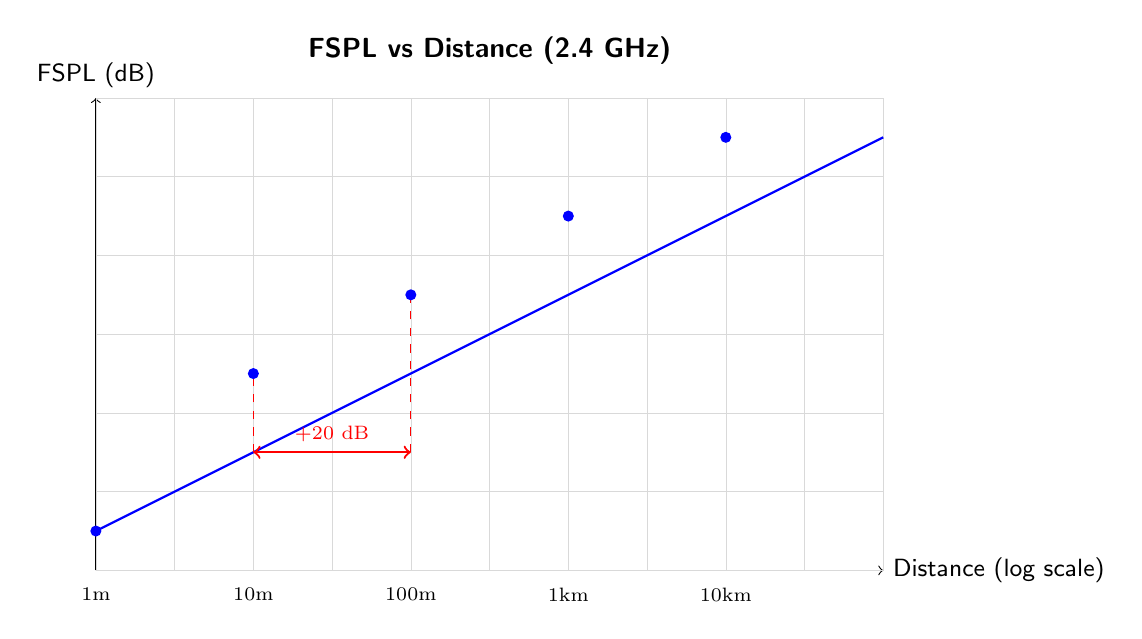
\begin{tikzpicture}[scale=1.0]
% Axes
\draw[->] (0,0) -- (10,0) node[right] {\sffamily\small Distance (log scale)};
\draw[->] (0,0) -- (0,6) node[above] {\sffamily\small FSPL (dB)};

% Grid
\draw[very thin,gray!30] (0,0) grid[step=1] (10,6);

% Log scale labels
\foreach \x/\label in {0/1m, 2/10m, 4/100m, 6/1km, 8/10km}
    \node[below, font=\scriptsize] at (\x,-0.1) {\label};

% Path loss line (20 dB/decade slope)
\draw[thick, blue] (0,0.5) -- (10,5.5);

% Annotations
\draw[<->, thick, red] (2,1.5) -- (4,1.5) node[midway, above, font=\scriptsize] {+20 dB};
\draw[dashed, red] (2,1.5) -- (2,2.5);
\draw[dashed, red] (4,1.5) -- (4,3.5);

% Title
\node[above, font=\sffamily\bfseries] at (5,6.3) {FSPL vs Distance (2.4 GHz)};

% Sample points
\foreach \x/\y in {0/0.5, 2/2.5, 4/3.5, 6/4.5, 8/5.5}
    \fill[blue] (\x,\y) circle (2pt);
\end{tikzpicture}
\end{center}

\subsection{Frequency Dependence}

From equation (9), FSPL increases with frequency:

\begin{equation}
\text{FSPL} \propto f^2 \quad \text{(power law)}
\end{equation}

In decibels: FSPL increases by \textbf{20~dB per decade} of frequency.

\textbf{Examples:}
\begin{itemize}
\item $100$~MHz $\rightarrow$ $1$~GHz: +20~dB loss
\item $1$~GHz $\rightarrow$ $10$~GHz: +20~dB loss
\item $10$~GHz $\rightarrow$ $100$~GHz: +20~dB loss
\end{itemize}

\textbf{Doubling frequency:} +6~dB loss (higher frequencies experience more path loss)

\textbf{Why?} Effective aperture of receiving antenna $A_{\text{eff}} \propto \lambda^2 \propto 1/f^2$ (smaller at higher frequencies).

\begin{center}
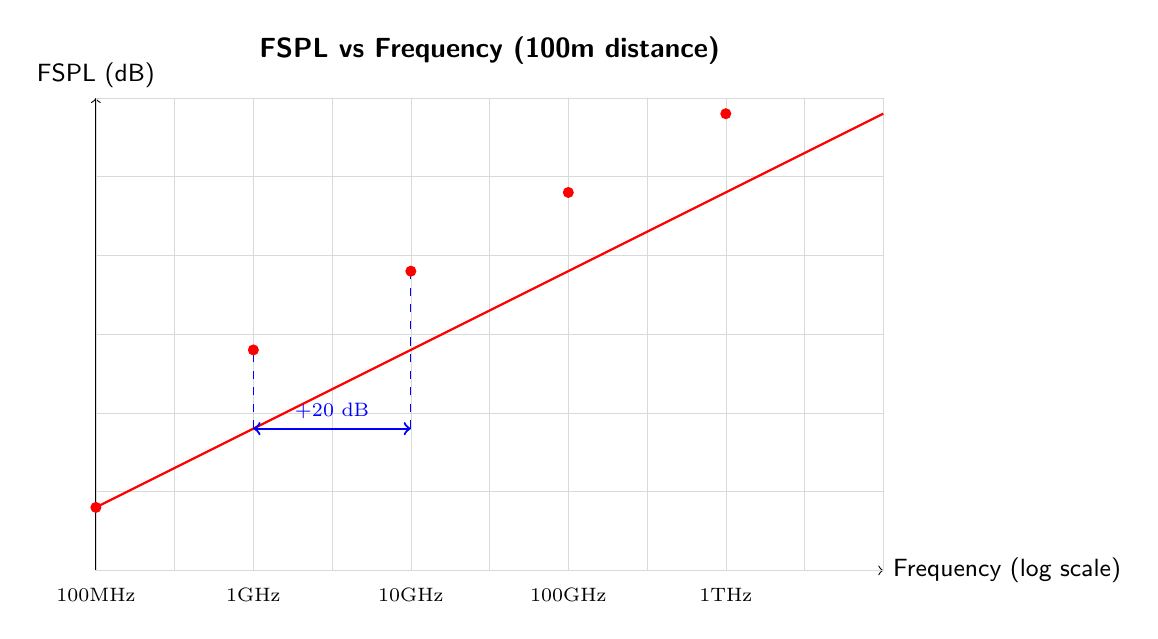
\begin{tikzpicture}[scale=1.0]
% Axes
\draw[->] (0,0) -- (10,0) node[right] {\sffamily\small Frequency (log scale)};
\draw[->] (0,0) -- (0,6) node[above] {\sffamily\small FSPL (dB)};

% Grid
\draw[very thin,gray!30] (0,0) grid[step=1] (10,6);

% Log scale labels
\foreach \x/\label in {0/100MHz, 2/1GHz, 4/10GHz, 6/100GHz, 8/1THz}
    \node[below, font=\scriptsize] at (\x,-0.1) {\label};

% Path loss line (20 dB/decade slope)
\draw[thick, red] (0,0.8) -- (10,5.8);

% Annotations
\draw[<->, thick, blue] (2,1.8) -- (4,1.8) node[midway, above, font=\scriptsize] {+20 dB};
\draw[dashed, blue] (2,1.8) -- (2,2.8);
\draw[dashed, blue] (4,1.8) -- (4,3.8);

% Title
\node[above, font=\sffamily\bfseries] at (5,6.3) {FSPL vs Frequency (100m distance)};

% Sample points
\foreach \x/\y in {0/0.8, 2/2.8, 4/3.8, 6/4.8, 8/5.8}
    \fill[red] (\x,\y) circle (2pt);
\end{tikzpicture}
\end{center}

\begin{keyconcept}
The $d^2 f^2$ relationship explains why:
\begin{itemize}
\item \textbf{Satellite links} at 36,000~km have enormous path loss (205~dB at 12~GHz)
\item \textbf{5G mmWave} (28~GHz) has 10~dB more loss than 4G LTE (2~GHz) at the same distance
\item \textbf{THz communications} are limited to very short ranges despite high bandwidth
\end{itemize}
\end{keyconcept}

\section{Link Budget Fundamentals}

The link budget equation combines transmitter power, antenna gains, and path loss:

\begin{equation}
P_R[\text{dBm}] = P_T[\text{dBm}] + G_T[\text{dBi}] + G_R[\text{dBi}] - \text{FSPL}[\text{dB}] - L_{\text{other}}[\text{dB}]
\end{equation}
where:
\begin{itemize}
\item $P_T$ = transmit power (dBm, referenced to 1~mW)
\item $G_T$, $G_R$ = antenna gains (dBi, referenced to isotropic)
\item FSPL = free-space path loss (dB)
\item $L_{\text{other}}$ = additional losses (cables, connectors, atmosphere, etc.)
\end{itemize}

\textbf{Design criterion:} For reliable communication, the received power must exceed the receiver sensitivity:
\begin{equation}
P_R \geq P_{\text{sens}} = N_0 + 10\log_{10}(B) + \text{SNR}_{\text{req}} + N_F
\end{equation}
where:
\begin{itemize}
\item $N_0 = -174$~dBm/Hz (thermal noise floor at 290~K)
\item $B$ = bandwidth (Hz)
\item $\text{SNR}_{\text{req}}$ = required SNR for target BER
\item $N_F$ = receiver noise figure (dB)
\end{itemize}

\subsection{\texorpdfstring{ Real-World
Deviations}{ Real-World Deviations}}\label{real-world-deviations}

\subsubsection{FSPL Assumes Free Space}\label{fspl-assumes-free-space}

\textbf{Reality}: - Atmosphere absorbs (especially water vapor at
mmWave/THz) - Obstacles block (buildings, trees, terrain) - Ground
reflections create multipath - Weather attenuates (rain, fog)

\textbf{Actual path loss} \textgreater{} FSPL

\begin{center}\rule{0.5\linewidth}{0.5pt}\end{center}

\subsubsection{Frequency-Specific
Effects}\label{frequency-specific-effects}

\textbf{Low Frequencies (\textless{} 30 MHz)}: - Ground wave propagation
- Ionospheric reflection - \textbf{Can exceed FSPL predictions} (longer
range!)

\textbf{Mid Frequencies (30 MHz - 3 GHz)}: - Mostly line-of-sight (LOS)
- FSPL + diffraction - Close to FSPL predictions

\textbf{High Frequencies (\textgreater{} 3 GHz)}: - Atmospheric
absorption becomes significant - Rain fade (especially \textgreater{} 10
GHz) - \textbf{Path loss \textgreater{} FSPL}

\textbf{THz (\textgreater{} 300 GHz)}: - Extreme atmospheric absorption
- Water vapor resonances - \textbf{Path loss \textgreater\textgreater{}
FSPL} (can be +100 dB extra!)

\begin{center}\rule{0.5\linewidth}{0.5pt}\end{center}

\subsection{\texorpdfstring{ Measurement
vs.~Prediction}{ Measurement vs.~Prediction}}\label{measurement-vs.-prediction}

\subsubsection{Received Power
Measurement}\label{received-power-measurement}

\begin{verbatim}
Measured:  P_R,meas
Predicted: P_R,pred (from Friis equation)

Path loss exponent n:
P_R  d^(-n)

Free space: n = 2
Urban: n = 3-4
Indoor: n = 4-6
\end{verbatim}

\textbf{Empirical models} (e.g., Okumura-Hata, COST 231) fit measured
data to more complex formulas.

\begin{center}\rule{0.5\linewidth}{0.5pt}\end{center}

\subsection{\texorpdfstring{ Key
Takeaways}{ Key Takeaways}}\label{key-takeaways}

\begin{enumerate}
\def\labelenumi{\arabic{enumi}.}
\tightlist
\item
  \textbf{FSPL \$\textbackslash propto\$
  d\textbackslash textsuperscript\{2\} \$\textbackslash cdot\$
  f\textbackslash textsuperscript\{2\}}: Geometric spreading, worse at
  high frequencies
\item
  \textbf{20 dB per decade}: Doubling d or f adds 6 dB loss
\item
  \textbf{Not energy loss}: Power spreads out, doesn\textquotesingle t
  vanish
\item
  \textbf{Baseline for link budgets}: Real losses are usually higher
\item
  \textbf{Frequency trade-off}: Higher f \$\textbackslash rightarrow\$
  more bandwidth but more path loss
\item
  \textbf{THz communications}: FSPL alone is \textasciitilde350 dB at 10
  m, 1 THz!
\end{enumerate}

\begin{center}\rule{0.5\linewidth}{0.5pt}\end{center}

\subsection{\texorpdfstring{ See Also}{ See Also}}\label{see-also}

\begin{itemize}
\tightlist
\item
  {[}{[}Maxwell\textquotesingle s-Equations-\&-Wave-Propagation{]}{]} -
  Theoretical foundation
\item
  {[}{[}Antenna-Theory-Basics{]}{]} - Antenna gain (G\_T, G\_R)
\item
  {[}{[}Link-Loss-vs-Noise{]}{]} - FSPL vs additive noise
\item
  {[}{[}Atmospheric Effects{]}{]} - Additional losses beyond FSPL
  \emph{(coming soon)}
\item
  {[}{[}Multipath-Propagation-\&-Fading-(Rayleigh,-Rician){]}{]} -
  Deviations from FSPL \emph{(coming soon)}
\item
  {[}{[}Terahertz-(THz)-Technology{]}{]} - Extreme FSPL regime
\end{itemize}

\begin{center}\rule{0.5\linewidth}{0.5pt}\end{center}

\subsection{\texorpdfstring{ References}{ References}}\label{references}

\begin{enumerate}
\def\labelenumi{\arabic{enumi}.}
\tightlist
\item
  \textbf{Friis, H.T.} (1946) ``A note on a simple transmission
  formula'' \emph{Proc. IRE} 34, 254-256
\item
  \textbf{Rappaport, T.S.} (2002) \emph{Wireless Communications:
  Principles and Practice} 2nd ed.~(Prentice Hall)
\item
  \textbf{Goldsmith, A.} (2005) \emph{Wireless Communications}
  (Cambridge UP)
\item
  \textbf{ITU-R P.525} (2019) ``Calculation of free-space attenuation''
\end{enumerate}
